\chapter{Cronograma}
\label{sec:cronograma}
A continuaci\'on se listan las actividades con su estimaci\'on de tiempo:
\begin{itemize}
\item Elecci\'on OCR: 8 d\'ias.
\item Dise\~no y desarrollo m\'odulo de preprocesamiento: 15 d\'ias.
\item Pruebas y ajustes m\'odulo de preprocesamiento: 5 d\'ias.
\item Estudio m\'etodos de b\'usqueda de texto: 25 d\'ias.
\item Selecci\'on m\'etodo de b\'usqueda: 8 d\'ias.
\item Ajustes al algoritmo de b\'usqueda: 15 d\'ias.
\item Dise\~no y desarrollo m\'odulo de coincidencias: 30 d\'ias.
\item Pruebas y ajustes al m\'odulo de coincidencias: 3 d\'ias.
\item Pruebas preliminares de la aplicaci\'on: 5 d\'ias.
\item Ajustes necesarios: 10 d\'ias.
\item Prueba piloto y validaci\'on: 10 d\'ias.
\item Escritura documento de proyecto: 20 d\'ias.

\end{itemize}
La figura \ref{fig:dgantt} contiene un diagrama Gantt del cronograma, empezando en enero 20 de 2014:
\begin{figure}[h]
\begin{center}
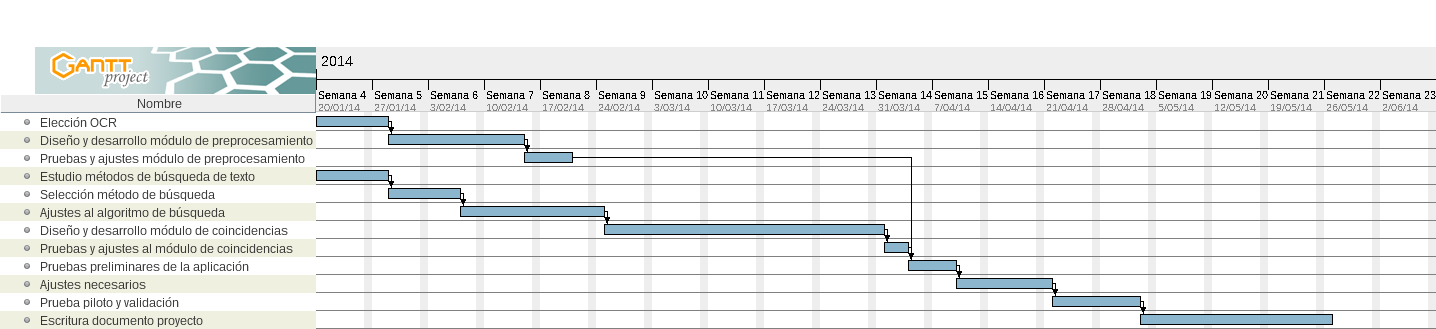
\includegraphics[scale=0.3]{./CronogramaProyectoGrado.png}
\end{center}
{\caption{Diagrama Gantt}\label{fig:dgantt}}
\end{figure}

\pagebreak